\documentclass[a4paper,12pt]{article}
\usepackage[margin=1in]{geometry}
\usepackage [utf8]{inputenc}
\usepackage{moreverb}
\usepackage{listings}
\usepackage{graphicx}
\usepackage{verbatim}
\usepackage{amsmath}
\usepackage{amsfonts}
\usepackage{lastpage}
\usepackage{url}
\usepackage{minted}

\usemintedstyle{colorful}

\usepackage{fancyhdr}
\pagestyle{fancy}
\lhead{Multi-Paradigm Assignment\\ TIPLPA}
\chead{26-05-2014 \\}
\rhead{Lasse Brøsted Pedersen\\ 10769 - Group 4}
\lfoot{}
\cfoot{}
\rfoot{Page \thepage ~of \pageref{LastPage}}

\DeclareGraphicsExtensions{.pdf,.png,.jpg}

\newcommand{\code}[1]{{\fontfamily{pcr}\selectfont #1}}

\begin{document}

\section{Functionality of the Application}

The application meets the requirements outlined in the assignment, and thus allows a user to input arbitrary, continuous, mathematical functions in the form of scheme procedure and have them, including derivative and integral plotted. Figure \ref{fig:screendump} shows the application in action. Highlights include:

\begin{itemize}
\item Syntax highlighting for scheme code.
\item Consistent color coding for each function and related dataseries (derivative, integral).
\item A log of output is associated with each function. Output includes stdout, stderr, syntax errors and other scheme errors.
\item Automatic conversion between step size and number of samples.
\item Updating axis values recalculates all functions if necessary.
\item Support for left-hand, middlepoint and right-hand integration.
\end{itemize}

\subsection{The User Interface}

\begin{figure}[h]
	\centering
	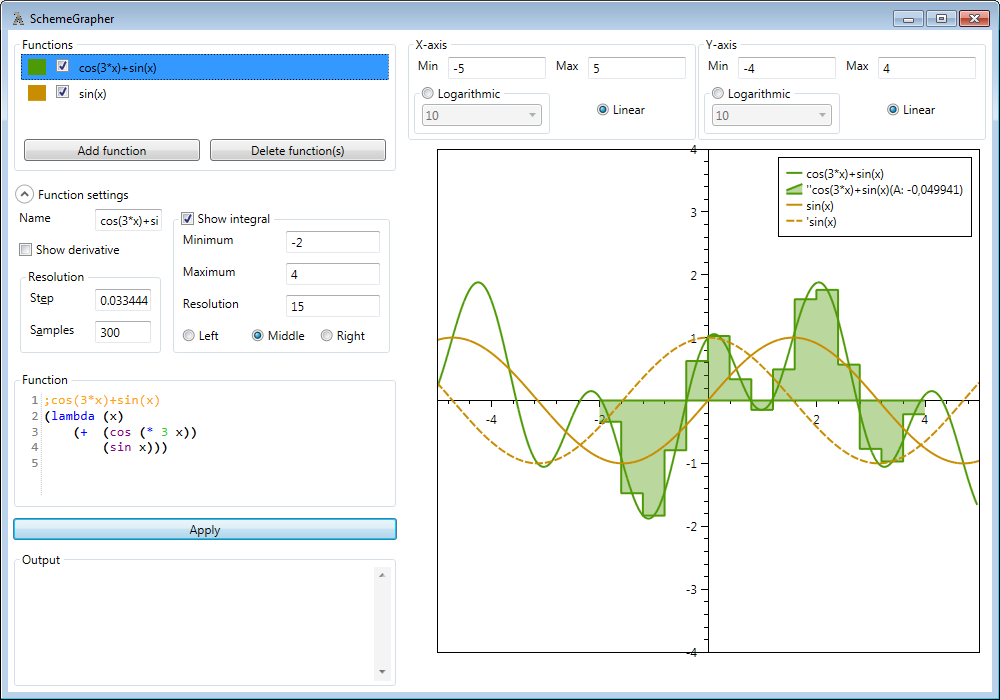
\includegraphics[scale=0.5]{schemegraphersscreen1}
	\caption{Screen dump showing various functionality of the application. }
    \label{fig:screendump}
\end{figure}

First of all, functions are managed from the function list in upper left corner. The list shows the name and color, and allows functions to be disabled/enabled. When a function is selected, its related properties are shown below.
The 'Function settings' box exposes settings for resolution of the function as either step size or number of samples, along with options for showing derivative and integral. The integral is calculated using the rectangle method, as either left, middle or right-hand.

The syntax highlighted scheme code associated with the function can be seen and edited below the settings box. This box is an editable textbox where the code for the corresponding chosen list item in the Function list is shown. The 'Apply' button below the box calculates and displays the function using the related settings. 
The last box in the left side is the Output box. In this box all the output from the applied code is written. This box is also for error messages for syntactical errors and other exceptions.
\\

The right side of the GUI is the Graph section. At the top, the minimum and maximum values of the X and Y axes can be changed, and also if the axes are to linear or logarithmic. Bases $log_2$, $log_{10}$ or $ln$ are available for logarithmic axes. Lastly, when an integral function is active, the associated legend shows the area of the integral approximation.

\section{Architecture}

As required by the assignment, the application is split into two parts: all mathematical calculations are handled in Scheme -  GUI and control flow of the program is handled by the (mostly) imperative language C\#. For this project, the scheme implementation used is IronScheme\footnote{\url{http://ironscheme.codeplex.com/}} which is implemented on the .NET platform, and thus integrates well with C\# and vice versa. The layers of the application is shown in figure \ref{fig:layers}.

\begin{figure}[h]
	\centering
	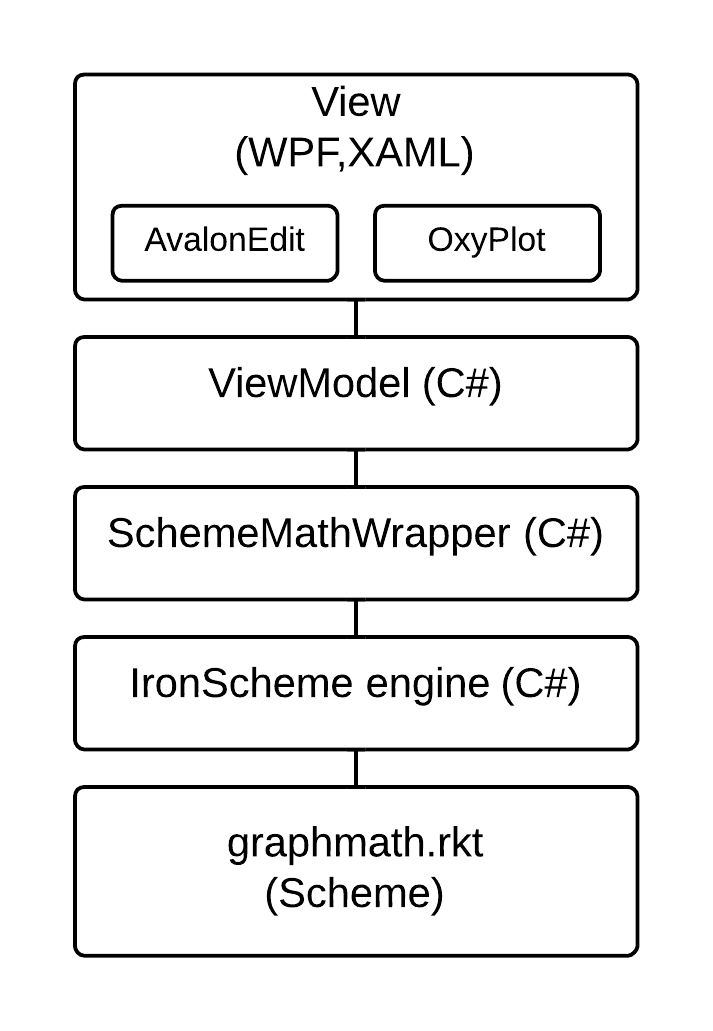
\includegraphics[scale=0.23]{MultiParadigmeBlocks}
	\caption{Layers of the application}
    \label{fig:layers}
\end{figure}

As figure \ref{fig:layers} shows, the application is based on .NET with a GUI written in WPF(Windows Presentation Foundation) using the Model-View-ViewModel(MVVM)-pattern. The view presents the graphical interface, and allows the user to interact with the application. AvalonEdit is a custom control for textediting that provides syntax highlighting, and OxyPlot is the charting control used. The ViewModel interacts with the model, the SchemeMathWrapper and presents data to the view.

\subsection{Bridging IronScheme and C\#}
 
The purpose of the SchemeMathWrapper is to provide the bridge between the imperative C\# application, and the functional Scheme procedures. Bridging involves translating from C\# function calls to Scheme procedure calls, and back and forth between native types of each paradigm.

\begin{listing}[H]
\begin{minted}[fontsize=\footnotesize, linenos]{csharp}
IEnumerable<Tuple<double, double>> CalcPlotData(string f, double min, double max, double step)
{
    var xyCons = "(calc-plot-data {0} {1} {2} {3})".Eval<Cons>(f.Eval(), min, max, step);

    //convert from Cons<Cons> (pseudo) to IEnumerable<Tuple<double, double>>
    return CreateListOfTuples(xyCons);
}
\end{minted}	

\caption{Bridging in \code{SchemeMathWrapper.CalcPlotData()}.}
\label{lst:SchemeCalcWrap}
\end{listing}

The C\# function in listing \ref{lst:SchemeCalcWrap} shows how bridging is done in the application. This particular function calculates the xy-coordinate pairs for the scheme procedure \code{f} passed as a string. The string \code{f} is evaluated to obtain a scheme procedure and passed to the evaluation of the scheme expression as argument \code{\{0\}}. Prior to using this function, the scheme procedure \code{calc-plot-data} has been loaded into the IronScheme engine by evaluating the contents of the file \code{schememath.rkt}, which contains regular scheme procedure definitions such as this one:

\begin{minted}[fontsize=\footnotesize]{scheme}
(define calc-plot-data
  (lambda (f min max step)
    ..
\end{minted}	

Evaluating the function returns a scheme list, represented as the C\# class \code{Cons} (part of IronScheme), where each \code{car} element is a \code{Cons}-pair containing a x and y value. Since IronScheme is based on .NET, it shares most data types (apart from \code{cons}) such as \code{string, int, double, array} and \code{Stream} with other .NET languages. IronScheme provides methods for converting back and forth between IronScheme procedures and .NET delegates allowing functions/procedures to be passed in both directions.

\subsection{User interaction}

The overall flow sequence of drawing a single function is a shown in figure \ref{fig:sequence}. The sequence shows the flow, from the user pressing apply on the UI to the plot being drawn.

\begin{figure}[h]
	\centering
	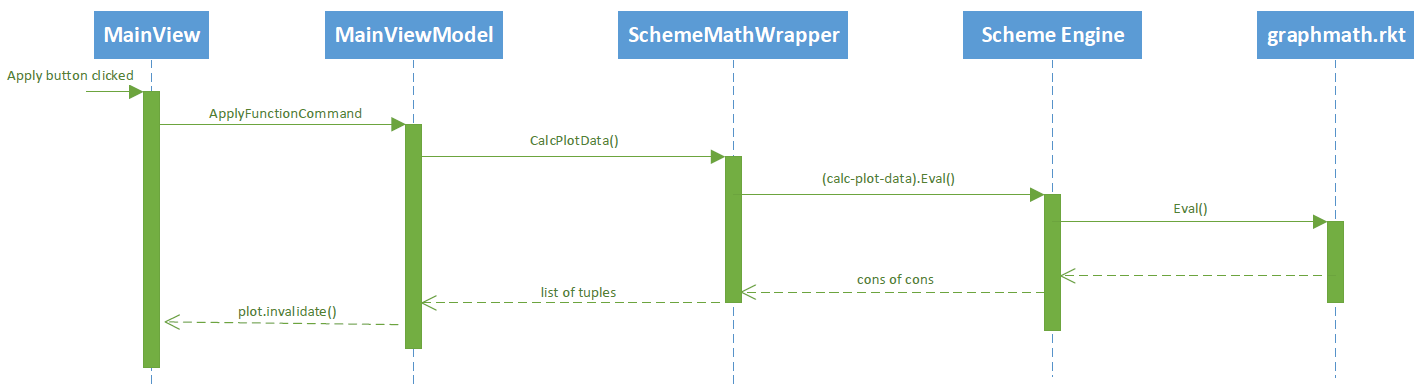
\includegraphics[scale=0.45]{sequence}
	\caption{Sequence diagram for calculating plot values (simplified)}
    \label{fig:sequence}
\end{figure} 

A shortcoming of the of the approach used in this application is the placement of validation of user input. MVVM is build around databindings from one object to another, with bound objects implementing error-reporting interfaces for validation. This concept is not well supported by scheme, so in this application validation of input data is mostly handled in the ViewModel.
		
\section{Testing Strategy}	
The application was tested by two test suites. One test suite was a .NET test written i C\# using the built-in test framework MSTest, which tests the C\# portion of the application. The other test suite was a unit test written in Scheme to test the business logic (ie. mathematical calculations) used for this application. 

The scheme test is performed using the standalone IronScheme interpreter, so as to not introduce any errors that may be caused by hosting IronScheme in a C\# application. 
Although unit test frameworks are available for scheme, none were used for this project, as having a framework was not essential for showing testing for this small application.

\begin{listing}[H]
\begin{minted}{scheme}
(define test:calc-plot-data 
  (equal? (calc-plot-data f 0 2 1/2) expected-plot-data))
\end{minted}	

\caption{Scheme test of \code{calc-plot-data}.}
\label{lst:SchemeTest}
\end{listing}

The C\# portion tested was primarily the C\# wrapper for the IronScheme code, since that is the central part of this application. The role of this test suite is to verify that the bridge works as expected, ie. correct scheme procedures are called with the correct arguments and the conversion to and from the data types of each language works as expected. The test of the wrapper is tested using the same (or equivalent) input and expected output as the pure scheme test to ensure correct behaviour. This however, leads to extra testing, because the same procedure/function is tested twice.

\begin{listing}[H]
\begin{minted}{csharp}
[TestMethod]
public void calcPlotData()
{
    var actual = SchemeMathWrapper.CalcPlotData(f, 0, 2, 0.5).ToList();

    CollectionAssert.AreEqual(expectedPlotData, actual);
}
\end{minted}	

\caption{Test of C\# wrapper for \code{calc-plot-data}.}
\label{lst:SchemeTest}
\end{listing}

Other parts of the application, in particular the ViewModel and  the GraphFunction class representing a single function and related properties should also be tested. These have not been tested in this project, but can be tested in the same manner as the IronScheme wrapper. 

	
\end{document}